\let\negmedspace\undefined
\let\negthickspace\undefined
\documentclass[journal]{IEEEtran}
\usepackage[a5paper, margin=10mm, onecolumn]{geometry}
\usepackage{tfrupee} 

\setlength{\headheight}{1cm}
\setlength{\headsep}{0mm}     

\usepackage{gvv-book}
\usepackage{gvv}
\usepackage{cite}
\usepackage{amsmath,amssymb,amsfonts,amsthm}
\usepackage{algorithmic}
\usepackage{graphicx}
\usepackage{textcomp}
\usepackage{xcolor}
\usepackage{txfonts}
\usepackage{listings}
\usepackage{enumitem}
\usepackage{mathtools}
\usepackage{gensymb}
\usepackage{comment}
\usepackage[breaklinks=true]{hyperref}
\usepackage{tkz-euclide} 
\usepackage{listings}
\def\inputGnumericTable{}                                 
\usepackage[latin1]{inputenc}                                
\usepackage{color}                                            
\usepackage{array}                                            
\usepackage{longtable}                                       
\usepackage{calc}                                             
\usepackage{multirow}                                         
\usepackage{hhline}                                           
\usepackage{ifthen}                                           
\usepackage{lscape}
\usepackage{circuitikz}


\tikzstyle{block} = [rectangle, draw, fill=blue!20, 
    text width=4em, text centered, rounded corners, minimum height=3em]
\tikzstyle{sum} = [draw, fill=blue!10, circle, minimum size=1cm, node distance=1.5cm]
\tikzstyle{input} = [coordinate]
\tikzstyle{output} = [coordinate]

\begin{document}

\bibliographystyle{IEEEtran}
\vspace{3cm}

\title{4.3.34}
\author{EE25BTECH11044 - Sai Hasini Pappula}
 \maketitle
{\let\newpage\relax\maketitle}

\renewcommand{\thefigure}{\theenumi}
\renewcommand{\thetable}{\theenumi}
\setlength{\intextsep}{10pt} 

\numberwithin{equation}{enumi}
\numberwithin{figure}{enumi}
\renewcommand{\thetable}{\theenumi}

\textbf{Question:}  
If the line 
\[
\frac{x}{a} + \frac{y}{b} = 1
\]
passes through the points $(2,-3)$ and $(4,-5)$, then find $(a,b)$. 

---

\textbf{Solution}

The line in intercept form is
\begin{equation}
\frac{x}{a} + \frac{y}{b} = 1.
\end{equation}
Substituting the points $\vec{x}_1=(2,-3)^T$ and $\vec{x}_2=(4,-5)^T$ yields
\begin{equation}
\frac{2}{a} - \frac{3}{b} = 1, \qquad
\frac{4}{a} - \frac{5}{b} = 1.
\end{equation}

Introduce unknowns
\begin{equation}
u=\frac{1}{a}, \quad v=\frac{1}{b},
\end{equation}
so the system becomes the linear matrix equation
\begin{equation}
\begin{bmatrix}
2 & -3\\[4pt]
4 & -5
\end{bmatrix}
\begin{bmatrix} u\\[2pt] v\end{bmatrix}
=
\begin{bmatrix}1\\[2pt]1\end{bmatrix}.
\end{equation}

Write the augmented matrix and perform Gauss--Jordan elimination:
\begin{equation}
\left[\begin{array}{cc|c}
2 & -3 & 1\\[4pt]
4 & -5 & 1
\end{array}\right]
\overset{R_2\leftarrow R_2-2R_1}{\longrightarrow}
\left[\begin{array}{cc|c}
2 & -3 & 1\\[4pt]
0 & 1 & -1
\end{array}\right]
\end{equation}
\begin{equation}
\overset{R_1\leftarrow R_1+3R_2}{\longrightarrow}
\left[\begin{array}{cc|c}
2 & 0 & -2\\[4pt]
0 & 1 & -1
\end{array}\right]
\overset{R_1\leftarrow \tfrac{1}{2}R_1}{\longrightarrow}
\left[\begin{array}{cc|c}
1 & 0 & -1\\[4pt]
0 & 1 & -1
\end{array}\right].
\end{equation}

Thus the solution for the unknown vector is
\[
\begin{bmatrix} u\\ v\end{bmatrix}
=
\begin{bmatrix} -1\\ -1\end{bmatrix}.
\]

Back-substitute $u=\dfrac{1}{a},\, v=\dfrac{1}{b}$:
\begin{equation}
\frac{1}{a}=-1 \Rightarrow a=-1,\qquad
\frac{1}{b}=-1 \Rightarrow b=-1.
\end{equation}

\textbf{Final Answer:}
\begin{equation}
(a,b)=(-1,-1),
\end{equation}
and the line becomes
\[
\frac{x}{-1}+\frac{y}{-1}=1 \quad\Longrightarrow\quad x+y=-1.
\]

\begin{center}
    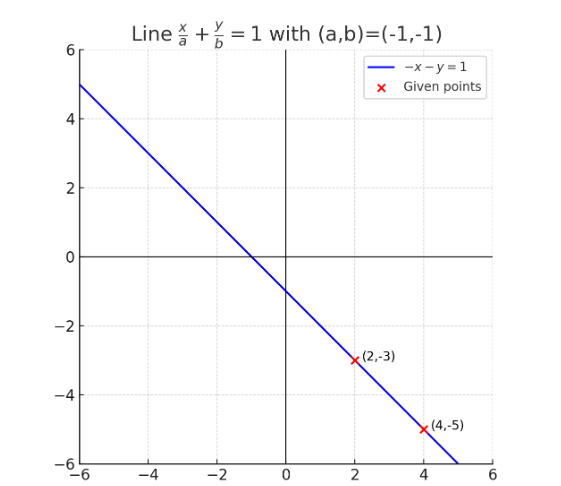
\includegraphics[width=0.8\columnwidth]{figs/plot6.png}
\end{center}

\end{document}
